
\chapter{Révisions et consolidation}
\section{Stratégie de révision}
\begin{retenir}
Une révision efficace alterne récupération en mémoire, correction explicite des erreurs et réemploi dans un problème. Relire passivement le cours ne suffit pas : il faut tenter une question sans modèle, comparer sa réponse, puis refaire la question après un délai.
\end{retenir}

Pour chaque chapitre, utiliser le code suivant : \textbf{V} (maîtrisé), \textbf{O} (fragile), \textbf{R} (à reprendre). Après le diagnostic, travailler en priorité une compétence orange ou rouge, puis vérifier immédiatement avec une question analogue.

\begin{center}
\begin{tabularx}{.9\textwidth}{lcccX}
\toprule
Compétence & V & O & R & Action de remédiation \\
\midrule
Choisir un modèle & $\square$ & $\square$ & $\square$ & Refaire un exercice de tri arithmétique/géométrique/exponentiel.\\
Lire et calculer & $\square$ & $\square$ & $\square$ & Reprendre les automatismes ciblés.\\
Rédiger et interpréter & $\square$ & $\square$ & $\square$ & Ajouter données, formule, calcul, unité et phrase de réponse.\\
\bottomrule
\end{tabularx}
\end{center}

\sessionheader{52}{11/05/2027}{B : 2 h -- C : 1 h}{Diagnostic des acquis}{Révisions et consolidation}
\begin{objectifs}\begin{itemize}\item Identifier les acquis.\item Classer les erreurs.\item Planifier la remédiation.\end{itemize}\end{objectifs}
\begin{automatismes}\begin{enumerate}\item Écrire le coefficient multiplicateur d'une hausse de $25\,\%$. \rep{$1+\dfrac{25}{100}=1,25$}\item Donner la formule du terme général arithmétique depuis $u_0$. \rep{$u_n=u_0+nr$}\item Résoudre $10^x=1000$. \rep{$x=3$}\item Dériver $x+\dfrac4x$. \rep{$1-\dfrac4{x^2}$}\item Énoncer la formule des probabilités totales avec deux branches. \rep{$P(B)=P(A)P_A(B)+P(\overline A)P_{\overline A}(B)$}\end{enumerate}\end{automatismes}
\begin{prerequis}Relire la dernière trace écrite et savoir effectuer les calculs élémentaires mobilisés aujourd'hui. Avant l'activité, faire reformuler les mots-clés : identifier les acquis et classer les erreurs.\end{prerequis}

\begin{activite}
Répondre sans cours à 14 questions, deux par chapitre. Reporter chaque erreur dans une grille : connaissance, choix de méthode, calcul, lecture, rédaction. Choisir ensuite deux priorités personnelles.

\end{activite}
\enseignant{La correction attend un profil d'erreurs et un plan de reprise, pas seulement une note globale. Faire verbaliser la donnée qui déclenche le choix de méthode.}

\begin{traceecrite}Le diagnostic sert à choisir la remédiation : reconnaître l'erreur, retrouver la règle utile, refaire une question analogue, puis vérifier sans aide.\end{traceecrite}

\begin{exemple}
Reprendre les données de l'activité et rédiger la solution dans l'ordre : définition des objets, propriété utilisée, calcul exact ou approché, puis phrase de réponse. La réponse modèle figure dans l'édition enseignant.
\end{exemple}
\enseignant{La correction attend un profil d'erreurs et un plan de reprise, pas seulement une note globale.}

\begin{exercice}[-- essentiel]
\begin{enumerate}\item Choisir entre suite arithmétique, suite géométrique et fonction exponentielle dans trois situations.\item Résoudre une équation exponentielle avec un logarithme.\item Calculer une probabilité à partir d'un arbre puis interpréter.\end{enumerate}
\end{exercice}
\enseignant{Justifier chaque choix par variation absolue ou relative ; vérifier la positivité avant le logarithme ; multiplier le long d'un chemin et conclure par une phrase.}

\manuelref{Réactivation des chapitres 1 à 7}
\ExoSession{52}

\begin{dm}Reprendre l'exercice d'entraînement 3 avec les données suivantes : remplacer la donnée initiale par $380$ et le taux ou la raison par $6$. Rédiger en quatre lignes : données, formule, calcul, conclusion.\end{dm}
\enseignant{La correction dépend de l'exercice repris. Vérifier surtout la cohérence du modèle, le nombre d'itérations, l'arrondi et la phrase de conclusion.}

\begin{sortie}Sur une demi-feuille : écrire la règle principale de la séance, traiter un exemple très court et indiquer son degré de confiance de 1 à 4. Question(s) essentielle(s) du jour : 1 et 2.\end{sortie}

\ifprof
\begin{methode}
\textbf{Conduite en 1 h :} 7 min d'automatismes ; 10 min de mise en commun et trace ; 28 min d'exercices essentiels ; 5 min de correction ; 3 min de billet de sortie.\\
\textbf{Conduite en 2 h :} ajouter 20 min de recherche de l'activité, 20 min d'institutionnalisation, un second exercice autonome et 10 min de correction comparée.\\
\textbf{Différenciation :} fournir aux élèves fragiles une fiche à quatre cases (données, modèle, calcul, conclusion). Demander aux élèves rapides de produire un contre-exemple, une justification ou une seconde méthode.
\end{methode}
\fi
\sessionheader{53}{13/05/2027}{B : 1 h -- C : 2 h}{Réactivation : fonctions exponentielles}{Révisions et consolidation}
\begin{objectifs}\begin{itemize}\item Réactiver les modèles exponentiels.\item Résoudre et interpréter.\item Contrôler les unités.\end{itemize}\end{objectifs}
\begin{automatismes}\begin{enumerate}\item Réduire $3x+7-x+2$. \rep{$2x+9$}\item Résoudre $10^x=1000$. \rep{$x=3$}\item Dériver $x+\dfrac4x$. \rep{$1-\dfrac4{x^2}$}\item Énoncer la formule des probabilités totales avec deux branches. \rep{$P(B)=P(A)P_A(B)+P(\overline A)P_{\overline A}(B)$}\item Donner la formule du terme général arithmétique depuis $u_0$. \rep{$u_n=u_0+nr$}\end{enumerate}\end{automatismes}
\begin{prerequis}Relire la dernière trace écrite et savoir effectuer les calculs élémentaires mobilisés aujourd'hui. Avant l'activité, faire reformuler les mots-clés : réactiver les modèles exponentiels et résoudre et interpréter.\end{prerequis}

\begin{activite}
Une valeur de $18\,000$ augmente de $3{,}5\,\%$ par an. Écrire le modèle, calculer la valeur après huit ans et déterminer quand elle dépassera $25\,000$.
\begin{center}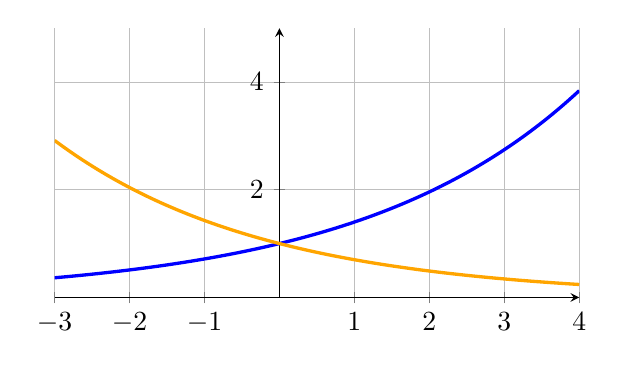
\begin{tikzpicture}\begin{axis}[width=.68\textwidth,height=5cm,axis lines=middle,xmin=-3,xmax=4,ymin=0,ymax=5,grid=major]\addplot[Blue,very thick,samples=100,domain=-3:4]{1.4^x};\addplot[Orange,very thick,samples=100,domain=-3:4]{.7^x};\end{axis}\end{tikzpicture}\end{center}
\end{activite}
\enseignant{$V(t)=18\,000\times1{,}035^t$, $V(8)\approx23\,703$. Le seuil est dépassé à partir de la dixième année. Faire verbaliser la donnée qui déclenche le choix de méthode.}

\begin{traceecrite}Une fonction exponentielle modélise une évolution relative constante. Identifier d'abord la valeur initiale et le coefficient multiplicateur.\end{traceecrite}

\begin{exemple}
Reprendre les données de l'activité et rédiger la solution dans l'ordre : définition des objets, propriété utilisée, calcul exact ou approché, puis phrase de réponse. La réponse modèle figure dans l'édition enseignant.
\end{exemple}
\enseignant{$V(t)=18\,000\times1{,}035^t$, $V(8)\approx23\,703$. Le seuil est dépassé à partir de la dixième année.}

\begin{exercice}[-- essentiel]
\begin{enumerate}\item Choisir entre suite arithmétique, suite géométrique et fonction exponentielle dans trois situations.\item Résoudre une équation exponentielle avec un logarithme.\item Calculer une probabilité à partir d'un arbre puis interpréter.\end{enumerate}
\end{exercice}
\enseignant{Justifier chaque choix par variation absolue ou relative ; vérifier la positivité avant le logarithme ; multiplier le long d'un chemin et conclure par une phrase.}

\manuelref{Calao, p. 48, n° 1 à 8, puis p. 54, n° 47 à 50}
\ExoSession{53}

\begin{dm}Reprendre l'exercice d'entraînement 2 avec les données suivantes : remplacer la donnée initiale par $385$ et le taux ou la raison par $7$. Rédiger en quatre lignes : données, formule, calcul, conclusion.\end{dm}
\enseignant{La correction dépend de l'exercice repris. Vérifier surtout la cohérence du modèle, le nombre d'itérations, l'arrondi et la phrase de conclusion.}

\begin{sortie}Sur une demi-feuille : écrire la règle principale de la séance, traiter un exemple très court et indiquer son degré de confiance de 1 à 4. Question(s) essentielle(s) du jour : 1, 2 et 3.\end{sortie}

\ifprof
\begin{methode}
\textbf{Conduite en 1 h :} 7 min d'automatismes ; 10 min de mise en commun et trace ; 28 min d'exercices essentiels ; 5 min de correction ; 3 min de billet de sortie.\\
\textbf{Conduite en 2 h :} ajouter 20 min de recherche de l'activité, 20 min d'institutionnalisation, un second exercice autonome et 10 min de correction comparée.\\
\textbf{Différenciation :} fournir aux élèves fragiles une fiche à quatre cases (données, modèle, calcul, conclusion). Demander aux élèves rapides de produire un contre-exemple, une justification ou une seconde méthode.
\end{methode}
\fi
\sessionheader{54}{18/05/2027}{B : 2 h -- C : 1 h}{Réactivation : logarithme décimal}{Révisions et consolidation}
\begin{objectifs}\begin{itemize}\item Réactiver les logarithmes.\item Résoudre une équation.\item Vérifier les conditions.\end{itemize}\end{objectifs}
\begin{automatismes}\begin{enumerate}\item Calculer $5\,\%$ de $160$. \rep{$8$}\item Dériver $x+\dfrac4x$. \rep{$1-\dfrac4{x^2}$}\item Énoncer la formule des probabilités totales avec deux branches. \rep{$P(B)=P(A)P_A(B)+P(\overline A)P_{\overline A}(B)$}\item Donner la formule du terme général arithmétique depuis $u_0$. \rep{$u_n=u_0+nr$}\item Résoudre $10^x=1000$. \rep{$x=3$}\end{enumerate}\end{automatismes}
\begin{prerequis}Relire la dernière trace écrite et savoir effectuer les calculs élémentaires mobilisés aujourd'hui. Avant l'activité, faire reformuler les mots-clés : réactiver les logarithmes et résoudre une équation.\end{prerequis}

\begin{activite}
Résoudre $10^x=340$, $1{,}06^n=2$ et $1{,}06^n\geq2$. Pour chaque réponse, distinguer valeur réelle, valeur approchée et rang entier minimal.

\end{activite}
\enseignant{$x\approx2{,}5315$ ; $n\approx11{,}90$ ; pour le seuil entier, $n=12$. Faire verbaliser la donnée qui déclenche le choix de méthode.}

\begin{traceecrite}Le logarithme transforme une équation exponentielle en équation sur l'exposant. Conditions : base positive différente de $1$, second membre positif.\end{traceecrite}

\begin{exemple}
Reprendre les données de l'activité et rédiger la solution dans l'ordre : définition des objets, propriété utilisée, calcul exact ou approché, puis phrase de réponse. La réponse modèle figure dans l'édition enseignant.
\end{exemple}
\enseignant{$x\approx2{,}5315$ ; $n\approx11{,}90$ ; pour le seuil entier, $n=12$.}

\begin{exercice}[-- essentiel]
\begin{enumerate}\item Choisir entre suite arithmétique, suite géométrique et fonction exponentielle dans trois situations.\item Résoudre une équation exponentielle avec un logarithme.\item Calculer une probabilité à partir d'un arbre puis interpréter.\end{enumerate}
\end{exercice}
\enseignant{Justifier chaque choix par variation absolue ou relative ; vérifier la positivité avant le logarithme ; multiplier le long d'un chemin et conclure par une phrase.}

\manuelref{Calao, p. 70, n° 1 à 10, puis p. 73 à 75, n° 30 à 42}
\ExoSession{54}

\begin{dm}Reprendre l'exercice d'entraînement 3 avec les données suivantes : remplacer la donnée initiale par $390$ et le taux ou la raison par $2$. Rédiger en quatre lignes : données, formule, calcul, conclusion.\end{dm}
\enseignant{La correction dépend de l'exercice repris. Vérifier surtout la cohérence du modèle, le nombre d'itérations, l'arrondi et la phrase de conclusion.}

\begin{sortie}Sur une demi-feuille : écrire la règle principale de la séance, traiter un exemple très court et indiquer son degré de confiance de 1 à 4. Question(s) essentielle(s) du jour : 1 et 2.\end{sortie}

\ifprof
\begin{methode}
\textbf{Conduite en 1 h :} 7 min d'automatismes ; 10 min de mise en commun et trace ; 28 min d'exercices essentiels ; 5 min de correction ; 3 min de billet de sortie.\\
\textbf{Conduite en 2 h :} ajouter 20 min de recherche de l'activité, 20 min d'institutionnalisation, un second exercice autonome et 10 min de correction comparée.\\
\textbf{Différenciation :} fournir aux élèves fragiles une fiche à quatre cases (données, modèle, calcul, conclusion). Demander aux élèves rapides de produire un contre-exemple, une justification ou une seconde méthode.
\end{methode}
\fi
\sessionheader{55}{20/05/2027}{B : 1 h -- C : 2 h}{Réactivation : fonction inverse}{Révisions et consolidation}
\begin{objectifs}\begin{itemize}\item Réactiver la fonction inverse.\item Mener une étude.\item Tracer et interpréter.\end{itemize}\end{objectifs}
\begin{automatismes}\begin{enumerate}\item Écrire le coefficient multiplicateur d'une hausse de $10\,\%$. \rep{$1+\dfrac{10}{100}=1,10$}\item Énoncer la formule des probabilités totales avec deux branches. \rep{$P(B)=P(A)P_A(B)+P(\overline A)P_{\overline A}(B)$}\item Donner la formule du terme général arithmétique depuis $u_0$. \rep{$u_n=u_0+nr$}\item Résoudre $10^x=1000$. \rep{$x=3$}\item Dériver $x+\dfrac4x$. \rep{$1-\dfrac4{x^2}$}\end{enumerate}\end{automatismes}
\begin{prerequis}Relire la dernière trace écrite et savoir effectuer les calculs élémentaires mobilisés aujourd'hui. Avant l'activité, faire reformuler les mots-clés : réactiver la fonction inverse et mener une étude.\end{prerequis}

\begin{activite}
Étudier $f(x)=x+\dfrac{16}{x}$ sur $]0,+\infty[$ et interpréter son minimum dans un contexte de coût moyen. Produire le tableau de variations et une esquisse.
\begin{center}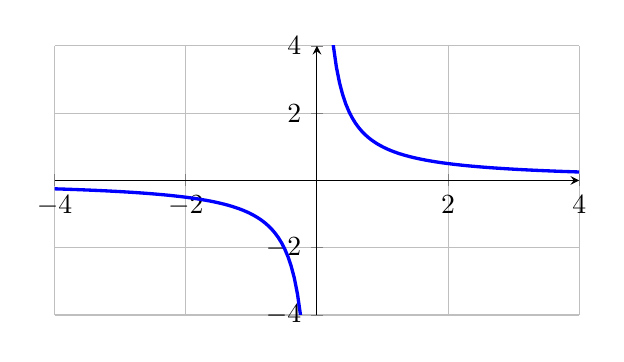
\begin{tikzpicture}\begin{axis}[width=.68\textwidth,height=5cm,axis lines=middle,xmin=-4,xmax=4,ymin=-4,ymax=4,grid=major]\addplot[Blue,very thick,samples=80,domain=-4:-.15]{1/x};\addplot[Blue,very thick,samples=80,domain=.15:4]{1/x};\end{axis}\end{tikzpicture}\end{center}
\end{activite}
\enseignant{$f'(x)=\dfrac{(x-4)(x+4)}{x^2}$ ; minimum $f(4)=8$. Faire verbaliser la donnée qui déclenche le choix de méthode.}

\begin{traceecrite}Pour une fonction contenant $\dfrac1x$, commencer par exclure $x=0$, puis dériver, factoriser et étudier le signe avant les variations.\end{traceecrite}

\begin{exemple}
Reprendre les données de l'activité et rédiger la solution dans l'ordre : définition des objets, propriété utilisée, calcul exact ou approché, puis phrase de réponse. La réponse modèle figure dans l'édition enseignant.
\end{exemple}
\enseignant{$f'(x)=\dfrac{(x-4)(x+4)}{x^2}$ ; minimum $f(4)=8$.}

\begin{exercice}[-- essentiel]
\begin{enumerate}\item Choisir entre suite arithmétique, suite géométrique et fonction exponentielle dans trois situations.\item Résoudre une équation exponentielle avec un logarithme.\item Calculer une probabilité à partir d'un arbre puis interpréter.\end{enumerate}
\end{exercice}
\enseignant{Justifier chaque choix par variation absolue ou relative ; vérifier la positivité avant le logarithme ; multiplier le long d'un chemin et conclure par une phrase.}

\manuelref{Calao, p. 94, n° 1 à 9, puis p. 96, n° 10 à 21}
\ExoSession{55}

\begin{dm}Reprendre l'exercice d'entraînement 2 avec les données suivantes : remplacer la donnée initiale par $395$ et le taux ou la raison par $3$. Rédiger en quatre lignes : données, formule, calcul, conclusion.\end{dm}
\enseignant{La correction dépend de l'exercice repris. Vérifier surtout la cohérence du modèle, le nombre d'itérations, l'arrondi et la phrase de conclusion.}

\begin{sortie}Sur une demi-feuille : écrire la règle principale de la séance, traiter un exemple très court et indiquer son degré de confiance de 1 à 4. Question(s) essentielle(s) du jour : 1, 2 et 3.\end{sortie}

\ifprof
\begin{methode}
\textbf{Conduite en 1 h :} 7 min d'automatismes ; 10 min de mise en commun et trace ; 28 min d'exercices essentiels ; 5 min de correction ; 3 min de billet de sortie.\\
\textbf{Conduite en 2 h :} ajouter 20 min de recherche de l'activité, 20 min d'institutionnalisation, un second exercice autonome et 10 min de correction comparée.\\
\textbf{Différenciation :} fournir aux élèves fragiles une fiche à quatre cases (données, modèle, calcul, conclusion). Demander aux élèves rapides de produire un contre-exemple, une justification ou une seconde méthode.
\end{methode}
\fi
